\section{Descripción del prototipo}
El prototipo actual busca que sea posible integrar los datos del caso de estudio a el cluster definido en el prototipo 1 que se encuentra en el capitulo \ref{cap:Cap3} \texttt{ Evaluación y definición de requerimientos de la red distribuida}.
\\
Una vez que los datos sean cargados a los nodos, se busca comprobar que el cluster siga funcionando correctamente y que se puedan hacer consultas sobre los datos que este almacena, comprobando con esto su accesibilidad, disponibilidad y correcta asignación de los mismos a la red.
\section{Análisis}
\subsection{Análisis de la adaptación de los datos a la red distribuida}
%explicar hadoop 
El archivo de datos correspondiente al caso de estudio cuenta con 21GB de texto plano. Debido a que se definió que cada nodo de datos/replica cuenta con al menos 40GB de almacenamiento.Los datos podrán ser almacenados en la red distribuida sin causar problemas de almacenamiento ya que estos son soportados por las capacidades definidas en el prototipo 1 que fueron establecidas contemplando esta condición.
% Los datos correspondientes podrán ser adaptados al ambiente creado sin mayores complicaciones ya que esto es algo que ya se tenia contemplado desde el prototipo 1.
\\
Para poder adaptar los datos del caso de estudio a la red distribuida creada con anterioridad se hará uso de Apache Hadoop. 
\\
Esto debido a que este cuenta con Hadoop Distributed File System (HDFS). HDFS  es  un  sistema  de  archivos  distribuido  y  tolerante  a  fallos. Funciona  sobre  el  
conjunto  de  los  nodos  de  un  cluster  de  Hadoop,  balanceando  la  carga  de  archivos   entre   las   máquinas   del   cluster,   de   forma   equitativa.   Gracias   a   su   
naturaleza  distribuida,  proporciona  alta  disponibilidad  y  altas  prestaciones  que  le  permiten ser capaz de manejar archivos de gran tamaño.
\\
por lo que, haciendo uso de este sistema de manejo de archivos y teniendo las capacidades de almacenamiento en los nodos de la red distribuida es posible afirmar que se puede adaptar sin complicaciones el archivo de datos del caso de estudio.

\section{Diseño}
\subsection{Diseño de la red distribuida con nodos de datos}
La red distribuida cuenta con 3 nodos de datos/replica y un nodo maestro, una vez que se apliquen las configuraciones correspondientes a la asignación de los datos en los nodos de datos/replica así como un algoritmo para probar que los datos asignados son accesibles, la red distribuida deberá verse como la que se muestra en la imagen \ref{fig:redi3}
\newpage
\begin{figure}[!htbp]
	\hypertarget{fig:redi3}{\hspace{1pt}}
	\begin{center}
		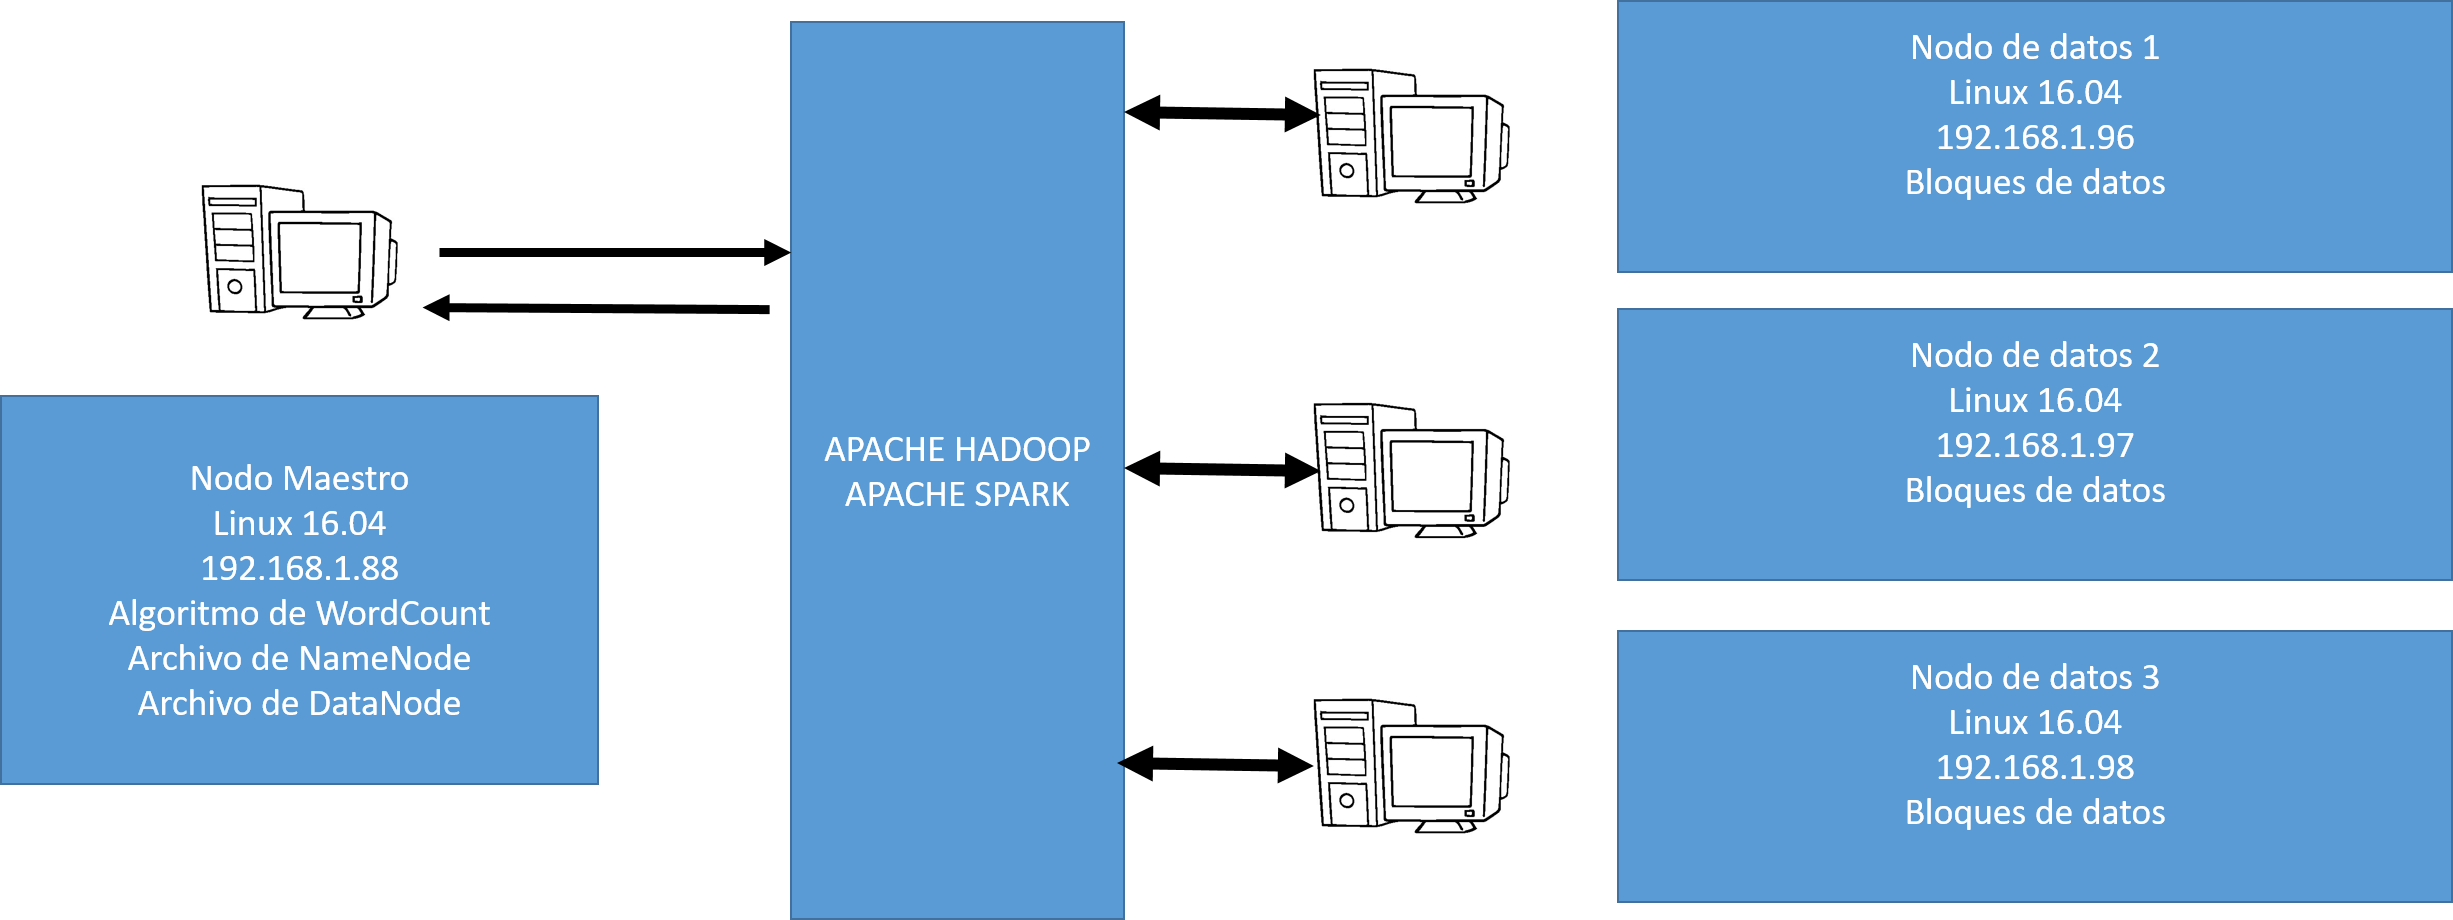
\includegraphics[width=.7\textwidth]{capitulo4/images/im3.png}
		\caption{Diseño de la red distribuida con nodos de datos}
		\label{fig:redi3}
	\end{center}
\end{figure}
la cual funciona conectando el cluster a una red local que les de una IP a cada uno de ellos la cual será definida como estática y se utilizara para las conexiones de manera distribuida tanto de Apache Hadoop como también de Apache Spark. 
\\
Los nodos de datos/replica no se comunicarán entre si al momento de ejecutar operaciones de computo en la red distribuida y para tal motivo utilizarán la conexión con el nodo maestro.
\\
%diagrama de como quedo constituida la red distribuida con apache hadoop y spark 
\subsection{Diseño de pruebas de obtención de información}
Para poder conocer si los datos fueron distribuidos correctamente y el cluster se encuentra en funcionamiento es posible utilizar un algoritmo que use los datos que se encuentran en el cluster y al final regrese un resultado.
\\
Los algoritmos de big data que serán necesarios para este trabajo son algoritmos que utilizan como base una tecnología llamada Map Reduce.
\\
Se encontró que existen algoritmos de prueba dentro de Hadoop que pueden ser utilizados para comprobar el correcto funcionamiento de la red. sin embargo, se busco comprender como es que estas pruebas funcionan.
\\
Y a su vez buscar que el ejemplo que sea aplicado sobre los datos del caso de estudio se adapte mejor a estos y ofrezca resultados mas interesantes.  
\\
\subsubsection{WordCount tradicional}
La prueba que se va a realizar es el "Contador de palabras" o "WordCount" este algoritmo lo que hace es contar todas las palabras que se encuentran dentro de un archivo y decir cuantas coincidencias de la misma palabra se encontraron. 
\\ 
El algoritmo funciona de la siguiente manera:
\begin{itemize}
\item Cada que encuentra una nueva palabra la agrega al listado de palabras con el valor de 1 que significa que solo ha sido encontrada una vez.
\item En caso de que la palabra sea encontrada nuevamente, entonces se reemplazara el número asociado a esa palabra por el número que tenia en ese momento + 1.
\item Termina cuando llega al final del archivo y por lo tanto todas las palabras nuevas fueron registradas y se conoce cuantas veces aparecen en el archivo.
\end{itemize} 
El procedimiento descrito anteriormente se explicará de igual forma con el diagrama de flujo que se muestra en la Imagen \ref{fig:redi}.

\begin{figure}[!htbp]
	\hypertarget{fig:redi}{\hspace{1pt}}
	\begin{center}
		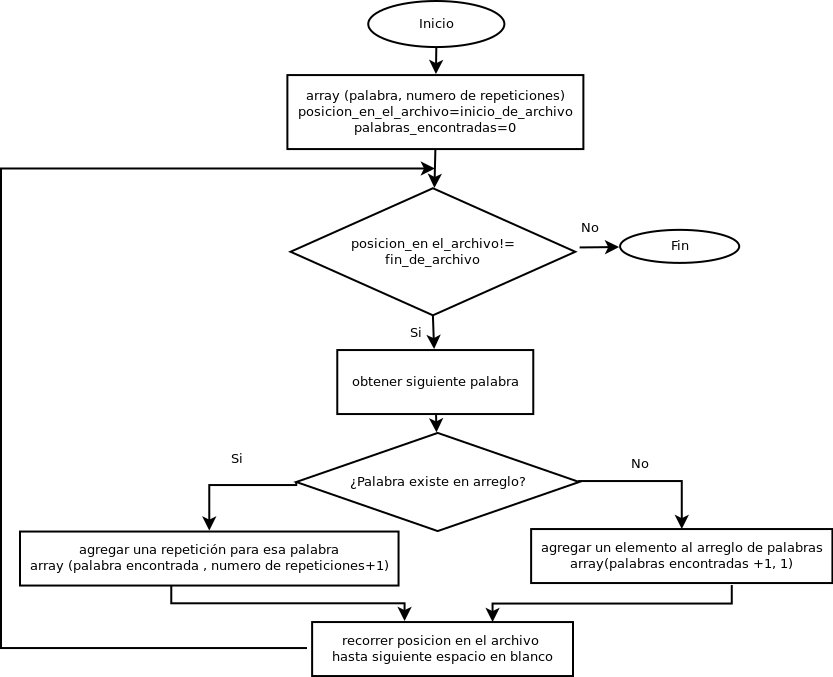
\includegraphics[width=.7\textwidth]{capitulo4/images/im1.png}
		\caption{Diagrama de flujo del algoritmo contador de palabras}
		\label{fig:redi}
	\end{center}
\end{figure}
Los pasos descritos anteriormente, son los pasos que serian utilizados si se tratara de un algoritmo que se ejecuta sin el uso de Map Reduce.
\subsubsection{WordCount con el uso de Map Reduce}
Map Reduce es una técnica que descompone un trabajo grande en tareas individuales las cuales pueden ser ejecutadas por separado en diferentes computadoras que componen un cluster, y estas al final pueden unir sus resultados individuales para calcular los resultados finales.
\\
\label{funcionmap}
\textbf{Función Map}: Toma un conjunto de datos y los convierte en otro conjunto de datos, donde los elementos individuales se dividen en entradas del nuevo conjunto con la estructura (clave-valor).
 \\
de tal forma que lo que una funcion Map en este ejemplo haría seria convertir el conjunto de palabras en un conjunto diferente donde:
Clave: toma el valor de la palabra que se encontró en el archivo
Valor: asigna el valor de 1 a otras las palabras encontradas en el archivo.
Veamos el siguiente conjunto de entrada dentro del archivo:
\begin{lstlisting} 
	botella, refresco, Botella, BOTELLA, Refresco,RefrescO, botellarefresco. 
\end{lstlisting} 
para este archivo el conjunto de salida de la funcion map, seria:
\begin{lstlisting} 
(botella,1), (refresco,1), (Botella,1), (BOTELLA,1),
 (Refresco,1),(RefrescO,1), (botellarefresco,1). 
\end{lstlisting} 
\label{funcionreduce}
\textbf{Función Reduce}: toma la salida del mapa y combina las entradas para generar un conjunto mas pequeño de datos
De tal forma que lo que la función reduce haría en este ejemplo seria buscar las palabras que sean las mismas de las entregadas por cada nodo y agruparlas. 
veamos el mismo ejemplo, suponiendo que el trabajo fue realizado por 3 nodos de datos, veamos lo que haría la función reduce.
\begin{lstlisting} 
nodo1
(botella,1), (refresco,1).
nodo2
(Botella,1), (BOTELLA,1).
nodo3
(Refresco,1),(RefrescO,1), (botellarefresco,1). 
\end{lstlisting} 
para estas entradas, el conjunto de salida de la función reduce seria:
\begin{lstlisting} 
(BOTELLA,3), (REFRESCO,3), (BOTELLAREFRESCO,1).
\end{lstlisting} 
Sin embargo, cabe destacar que el sistema de Hadoop no solo trabaja con las funciones map y reduce, sino que tiene otras funciones internas que el sistema controla.
\\
En la imagen \ref{fig:redi2} se puede visualizar el funcionamiento completo que tendría que ejecutarse en el cluster para llevar a cabo este algoritmo.
\begin{figure}[!htbp]
	\hypertarget{fig:redi2}{\hspace{1pt}}
	\begin{center}
		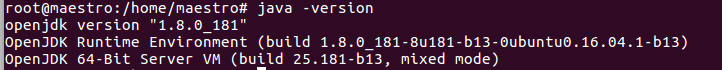
\includegraphics[width=.9\textwidth]{capitulo4/images/im2.png}
		\caption{Funcionamiento completo de Hadoop, con todas sus operaciones}
		\label{fig:redi2}
	\end{center}
\end{figure}
Teniendo como referencia la imagen \ref{fig:redi2} se explicarán los módulos que ejecuta Hadoop de forma interna para una aplicación Map Reduce de forma breve.
\begin{enumerate}
	\item \textbf{Partición}: Se requiere definir un parametro de partición, esto para que se puedan reconocer las unidades a analizar y con esto poder asignar tareas a los nodos. el parámetro de partición puede ser cualquier cosa, por ejemplo, dividir por espacio, coma, punto y coma, o incluso por una nueva línea ('\ n').
	\item \textbf{Mapeo}: Se explico anteriormente en \ref{funcionmap} \texttt{Función Map}.
	\item \textbf{Partición intermedia}:Se busca generar grupos con los datos que después de pasar por el modulo de mapeo y tener la estructura de salida de este modulo tienen la misma CLAVE, al cumplir esta condición se asignan en el mismo grupo. Se generan tantos grupos como claves existan.
	\item \textbf{Reducción}: Se explico anteriormente en \ref{funcionreduce} \texttt{Función Reduce}. 
	\item \textbf{Combinación}: Todos los datos de salida que arrojo la función de reducción son combinados y puestos en un solo grupo para generar un resultado final.
\end{enumerate}

\section{Desarrollo}
Para que Instalar Apache Hadoop en la red distribuida en funcionamiento se siguió el Manual de Instalación de Luminus 
en sus secciones 
\begin{verbatim}
4. Instalación de Apache Hadoop en el nodo maestro
	4.1. Instalación de Hadoop 
		4.1.1. Configuración
		4.1.2. Archivos de configuración
5. Instalación de Apache Hadoop en los nodos de datos
	5.1. Instalación de Hadoop en los nodos de datos 
		5.1.1. Configuración 
6. Puesta en funcionamiento
	6.1. Puesta en funcionamiento del Cluster manejado por el Servidor Apache Hadoop
\end{verbatim}
Las cuales nos permitirán instalar Apache Hadoop
% para permitir la conexión entre los nodos de datos/replica y el maestro haciendo uso de una red de internet local en la que se encuentren conectados todos los nodos.
%Además de contener todas las configuraciones necesarias para tal objetivo.  
%como se instala hadoop
%como rayos se hace el algoritmo (desde java)
\section{Pruebas}
%como se ve cuando lo ejecutas el algoritmo 